% 请确保文件编码为utf-8,使用XeLaTex进行编译,或者通过overleaf进行编译

\documentclass[answers]{exam}  % 使用此行带有作答模块
% \documentclass{exam} % 使用此行只显示题目

\usepackage{xeCJK}
\usepackage{zhnumber}
\usepackage{graphicx}
\usepackage{hyperref}
\usepackage{amsmath}
\usepackage{amssymb}
\usepackage{mathtools}
\usepackage{booktabs}
\usepackage{enumerate}
\usepackage{enumitem} % 控制列表样式
\usepackage{listings} 

\title{2025自然语言处理 \\ 课程设计1}
\date{2025.4.1}
\pagestyle{headandfoot}
\author{人工智能学院 221300079 王俊童}
\firstpageheadrule
\firstpageheader{南京大学}{2025自然语言处理}{课程设计1}
\runningheader{南京大学}
{2025自然语言处理}
{课程设计1}
\runningheadrule
\firstpagefooter{}{第\thepage\ 页(共\numpages 页)}{}
\runningfooter{}{第\thepage\ 页(共\numpages 页)}{}

% no box for solutions
% \unframedsolutions
\def \x \mathbf{x}


\setlength\linefillheight{.5in}

% \renewcommand{\solutiontitle}{\noindent\textbf{答:}}
\renewcommand{\solutiontitle}{\noindent\textbf{解:}\par\noindent}

\renewcommand{\thequestion}{\zhnum{question}}
\renewcommand{\questionlabel}{\thequestion .}
\renewcommand{\thepartno}{\arabic{partno}}
\renewcommand{\partlabel}{\thepartno .}

% 实验报告需包含以下内容:

% 实现了哪些方法并对自己设计的代码模块用简洁的语言描述
% 如何复现主要实现结果,包括执行命令和环境依赖,
% 建议修改requirement.txt和新建bash文件来展示如何运行代码
% 不同方法的实验结果如何
% 遇到的具体问题,如何解决
% 对该任务和在探索过程中的思考


\begin{document}
% \normalsize
\maketitle
综述,首先观察代码结构,逻辑如下:
\begin{itemize}
    \item 命令行参数解析。有method,是否analyze,statistical里面方法的选取。
    \item 加载数据和数据分析(需要我们实现数据分析)
    \item 三个方法的训练:
    \begin{itemize}
        \item rule:基于一些规则得到的一个实现。train有四种纠错规则:
        \begin{itemize}
            \item $\_extract\_confusion\_pairs$:字符混淆对提取。
            \item $\_extract\_punctuation\_rules$:标点符号规则提取
            \item $\_extract\_grammar\_rules$:语法规则提取
            \item $\_extract\_word\_confusion$:词汇混淆对提取
        \end{itemize}
        然后以上四种错误的纠错发生在correct里面。
        \item statistical:基于统计学习方法的纠错。这个里面又分为两个模型:
        \begin{itemize}
            \item ngram模型:初始化了一堆数据结构,1-4的gram方法,字符混淆矩阵和错误率等
            \item ml模型:用机器学习方法去做。
        \end{itemize}
        \item 集成学习方法,在框架代码的ensemble部分有留给我们实现。
    \end{itemize}
    \item 三个方法对应的纠错和评估。跟上面一样了,可以实现很多的correct方法,都有对应接口。
\end{itemize}
可以看出整个代码框架都还是比较整齐的,我们需要完成的TODO任务如下:
\begin{itemize}
    \item 数据的analyze分析部分和画图。
    \item rule:完成规则方法的实现。完成对应规则方法的纠错改正。
    \item statistical:完成ngram和ml方法的对应修正和改正。
    \item main:完成集成学习方法。
    \item 其余可以加一些深度学习之类的方法实现。
\end{itemize}

\section{实现方法及其简单描述,遇到的问题和解决方案(全包含,就不单独列了,按照我的编程和问题思考思路来写的)}
\subsection{数据分析部分}
数据分析部分,我们将原来的args做了一点点修改,然后我们首先可以根据原词典数据进行统计,把label为1的错误数据中的错误字符全部统计
出来,而且可以得到错误率最高的10个的错误模式和错误字符,这更方便我们后续处理:
\begin{lstlisting}
# 只看错的
if label == 1:  
    error_count += 1
    
    if len(source) == len(target):  
        for i, (s_char, t_char) in enumerate(zip(source, target)):
            if s_char != t_char:
                char_error_freq[s_char] += 1
                error_patterns[(s_char, t_char)] += 1
\end{lstlisting}
然后我们把它可视化, 同时,由于matplotlib不支持中文字体,需要更换自己电脑里面的路径。这个在对应
data analysis的python文件里面有讲。

可以看一个我做出来的效果,还是蛮不错的。
\begin{figure}[h]
    \centering
    \label{error_distribution}
    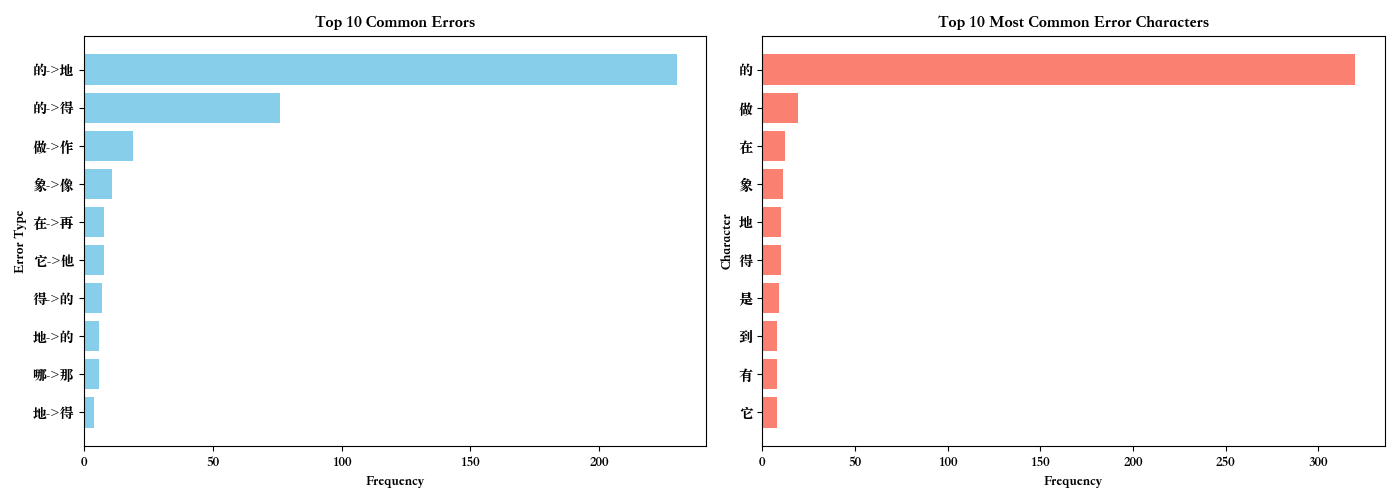
\includegraphics[width=1\textwidth]{../pic/error_distribution.png} 
    \caption{error distribution}  
\end{figure}
可以看到的和地的错误最多,还有的和得之类的,一般都是些同音不同意的字。

\subsection{3个方法部分}
\subsubsection{方法1:rule}
rule这个方法还蛮简单的,基本是基于人类的常识性的方法,有点像是打表。但是肯定有补全不了的规则,这个是硬伤。
共有如下的需要填补的方法:
\begin{itemize}
    \item self.\_extract\_confusion\_pairs:这个方法已经给我们补全了。意思是提取了混淆字符对。
    但是这个一眼就存在一些问题:
    \begin{itemize}
        \item 没有考虑插入和删除的错误
        \item 没有考虑很强烈的上下文特征
        \item 不同的count对于噪声过滤效果不一样,可以产生不一样的效果
    \end{itemize}
    我们首先修改这个混淆对的做法:
    
    \item self.\_extract\_punctuation\_rules
    \item self.\_extract\_grammar\_rules
    \item self.\_extract\_word\_confusion
\end{itemize}


\subsection{其余方法}

\section{如何复现结果和代码环境依赖问题}

\section{不同实验方法的对比结果}

\section{一些简单思考}

\end{document}